\graphicspath{{01-Introduction/Figures/}}

\section{Introduction}
\label{Sect:Intro}

Stored muon beams have been proposed as the basis of a facility
capable of delivering lepton-antilepton collisions at very high
energy~\cite{Neuffer:1994bt,Palmer:2014nza} and as the source of
uniquely well-characterised neutrino 
beams~\cite{Geer:1998PhRvD..57.6989G,Bandyopadhyay:2007kx,Apollonio:2002en}.
In the majority of designs for such facilities the muons are produced
from the decay of pions created when an intense proton beam strikes a
target.
The phase-space volume occupied by the tertiary muon beam must be
reduced (cooled) before it is accelerated and subsequently injected
into the storage ring.
The times taken to cool the beam using techniques that are presently in
use at particle accelerators (synchrotron-radiation cooling
\cite{2012acph.book.....L}, laser
cooling~\cite{PhysRevLett.64.2901,PhysRevLett.67.1238,doi:10.1063/1.329218},
stochastic cooling~\cite{Marriner:2003mn}, and electron
cooling~\cite{1063-7869-43-5-R01}) are long when compared with the
lifetime of the muon.
%The use of such techniques would therefore lead to unacceptably large
%losses through decay.
Ionization cooling~\cite{cooling_methods,Neuffer:1983jr}, in which a
muon beam is passed through a material (the absorber), where it
loses energy, and is then re-accelerated, occurs on a timescale short
compared with the muon lifetime.
Ionization cooling is therefore the only technique available to cool the muon beam at a neutrino factory or muon collider.
The international Muon Ionization Cooling Experiment (MICE)
provided the proof-of-principle demonstration of the
ionization-cooling technique~\cite{Bogomilov:2019kfj}.

MICE operated at the ISIS neutron and muon source at the STFC
Rutherford Appleton Laboratory from 2008 to 2018.  
The ISIS synchrotron accelerates protons to a kinetic energy of 800\,MeV at a repetition rate of
50\,Hz.
For MICE operation, a titanium target was dipped
%nearly once per second
into the halo of the proton beam with a rate of 0.78\,Hz. 
Pions created in the interaction were captured in a quadrupole triplet
(see figure~\ref{fig:BL}).
A beam line composed of dipole, solenoid, and quadrupole
magnets captured muons produced through pion decay and transported the
resulting muon beam to the MICE apparatus.
The momentum of the muon beam was determined by the settings of the two dipole magnets D1 and D2.
The emittance of the beam injected into the experiment was tuned using
a set of adjustable tungsten and brass diffusers.
The cooling cell was composed of a liquid hydrogen or lithium hydride
absorber placed inside a focus coil (FC) module, sandwiched between
two scintillating-fibre trackers (TKU, TKD) placed in superconducting
solenoids (SSU, SSD).
Together, SSU, FC, and SSD formed the magnetic channel.
The MICE coordinate system is such that the $z$-axis is coincident
with the beam direction, the $y$-axis points vertically upwards, and the
$x$-axis completes a right-handed co-ordinate system.

\begin{figure}[htb!]
  \begin{center}
    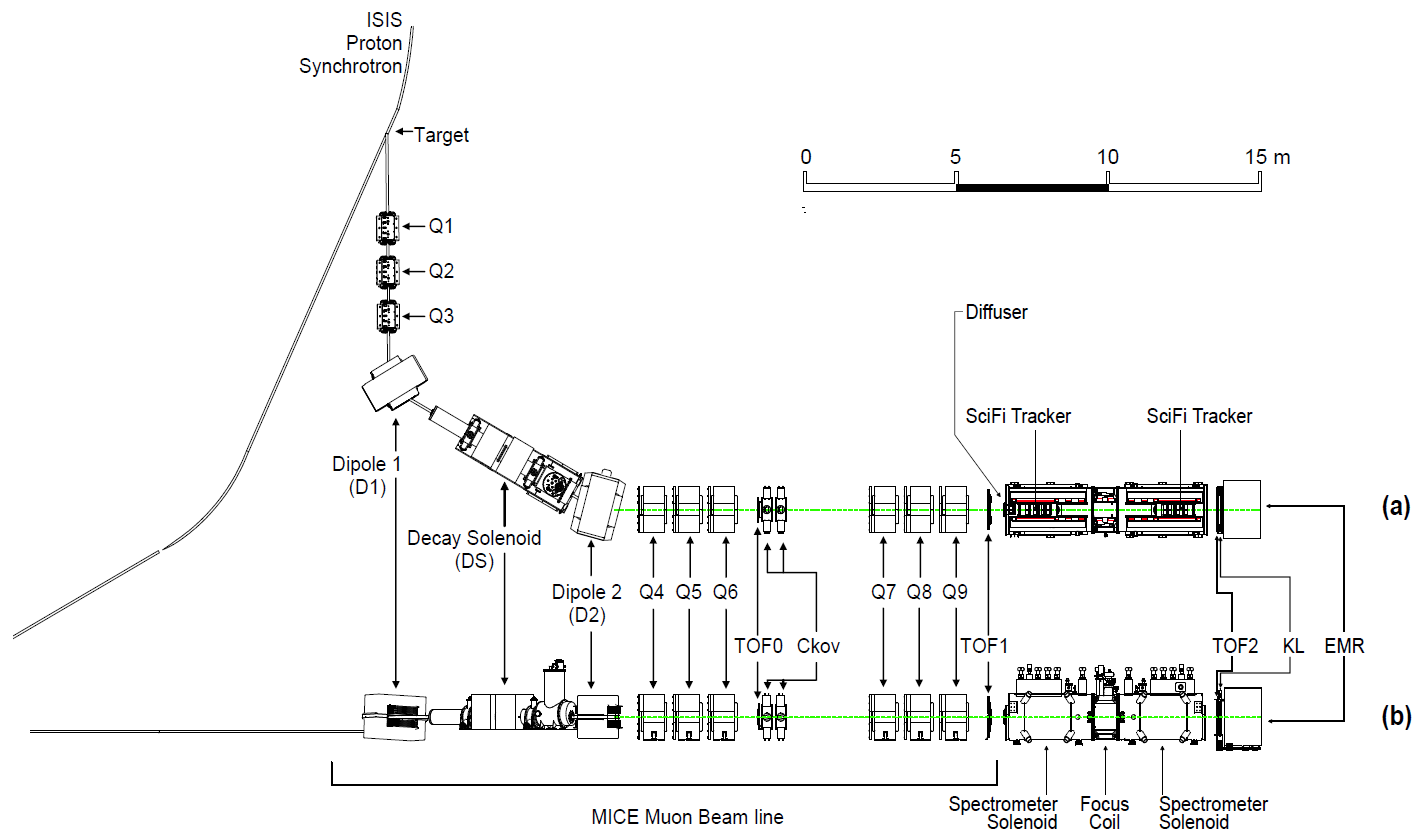
\includegraphics[width=1.0\columnwidth]{BL.png}
    \caption{
      MICE, top (a) and side (b) views, showing the full beam line
      starting from the target position on the proton synchrotron with the quadrupoles and dipoles (Q1 to Q9, D1, D2), the
      Decay Solenoid, and instrumented magnetic channel elements
      (including the trackers upstream, TKU, and downstream, TKD, of the cooling
      channel, placed inside superconducting solenoids, respectively SSU and SSD) with all the
      other PID detectors (three TOF stations, two Ckov detectors, KL and
      the EMR).
      The cooling cell, defined to be the liquid hydrogen absorber
      vessel inside the focus coil (FC), is shown in figure~\ref{Fig:AbsorberVessel:Diag}.
    }
    \label{fig:BL}
  \end{center}
\end{figure}

MICE measured the passage of single particles through the apparatus which were aggregated into
a beam offline.
This paper documents the performance of the instrumentation which was
used to fully characterise the beam, its evolution across the magnetic
channel.
The instrumentation used to quantify the physical properties of the liquid hydrogen absorber are also documented.
The instrumentation consisted of three time-of-flight detectors
(TOF0, TOF1, TOF2) discussed in section~\ref{Sect:TOF}, two 
threshold Cherenkov counters (CkovA, CkovB) discussed in
section~\ref{Sect:Ckov}, a sampling calorimeter (KL) discussed in
section~\ref{Sect:KL}, a tracking calorimeter (EMR) discussed in
section~\ref{Sect:EMR}, and the scintillating-fibre trackers
(section~\ref{Sect:Tracking}).
The properties of the the liquid hydrogen
absorber are described in ~\ref{Sect:Absorber}.
